\chapter{State of the Art} \label{chap:state_of_the_art}


\section*{Introduction}
Electricity grids, commonly referred to as “grids,” play a vital role in modern energy infrastructure. They facilitate power generation, transmission, distribution, and control. Over time, grids have evolved from localized systems to interconnected networks, adapting to meet increasing demands and technological advancements. These grids contribute significantly to economic and societal progress.

Amidst dynamic changes in the energy landscape, the emergence of the “smart grid” presents transformative possibilities. Leveraging data, automation, and connectivity, smart grids enhance energy management and promote sustainability. In this chapter, we delve into the evolution of grid systems and explore the challenges and opportunities associated with smart grid technology, shaping the future of energy.
\newpage


\section{Definition smart grid}
The Smart Grid is a comprehensive electrical network that employs cutting-edge communication technologies, computational intelligence, and cybersecurity protocols throughout the entire process of generating, transmitting, distributing, and consuming electricity. Its objective is to establish a system that is environmentally friendly, secure, dependable, adaptable, energy-efficient, and environmentally sustainable. While the ultimate vision of the Smart Grid is ambitious, its practical implementation demands careful evaluation of costs, rigorous testing, and validation. Introducing new functionalities can occur autonomously, with each necessitating justification and a reasonable return on investment. The compatibility of open systems facilitates smooth integration into the Smart Grid once the technologies have been validated.\cite{gharavi2011smart}


\subsection{Smart grid attributes}
Many smart grid advocates cite some or all of its following attributes as representative of its promise:
\firmlist
\begin{itemize}


\item \textbf{  Efficiency:} Capable of meeting growing consumer demand without the need for additional infrastructure.

\item \textbf{  Flexibility: }Able to accept energy from various sources, including solar and wind, with the same ease as traditional fuels like coal and natural gas. It can integrate new technologies, such as energy storage, as they become commercially viable.

\item \textbf{  Empowering: }Facilitating real-time communication between consumers and utility providers, allowing consumers to adjust their energy usage based on factors like price and environmental concerns.

\item \textbf{  Opportunistic:} Creating new markets and opportunities by leveraging plug-and-play innovations whenever suitable.

\item\textbf{   Focus on Quality:} Able to deliver reliable power without disruptions, ensuring the smooth operation of digital technologies crucial to our economy.

\item \textbf{  Resilience:} Increasingly resistant to cyber attacks and natural disasters through decentralization and the implementation of smart grid security measures.

\item \textbf{  Environmental Sustainability:} Contributing to the mitigation of climate change and offering a viable path towards reducing the environmental impact of electricity generation. \cite{el2014smart}
\end{itemize}

\section{Differences between Traditional grid and Smart grid }
Table 1.1 offers a thorough comparison of the conventional power grid with the smart grid. In contrast to the traditional grid where customers play a passive role, the smart grid actively engages them through bi-directional communication technologies. For instance, rooftop photovoltaic solar panels produce electricity during the day, enabling customers to sell surplus energy back to the grid. At night, these panels continue to power home appliances as usual. Moreover, the smart grid incorporates innovative technologies like distributed generation, electric vehicle charging and discharging, and Flexible Alternating Current Transmission Systems (FACTS) to improve energy distribution and management.\cite{zhang2014smart}
\begin{table}[h]
  
	\caption{Comparison between conventional grid and smart grid \cite{miller2008understanding}}
    

	\begin{tabular}{|p{3cm}|p{6cm}|p{6cm}|}
	\hline
	Aspects & Conventional Grid & Smart Grid \\
	\hline
	Interaction between Grid and Customers & Customers passively accept service from grid & Customers participation on the grid action \\
	\hline
	Renewable Energy Integration & Having trouble with renewable penetration & Integration with renewable resources enhancement \\
	\hline
	Options for Customers & No choice for customer, monopoly market & With digital market trading, PHEV, introduce bids and competition, more choice for customer \\
	\hline
	Options on Power Quality (PQ) & No choice on power quality, no price plan options for consumers & Power quality levels for different consumers \\
	\hline
	System Operation & Ageing power assets, no efficient operation & Assets operating optimization, less power loss \\
	\hline
	Protection & Only rely on protection devices, fault detect manually & Have capability of self-healing, less damage affected by fault \\
	\hline
	Reliability and Security & Susceptible to physical and cyber attack & More reliable for national security and human safety \\
	\hline
	\end{tabular}

	\label{tab:my_label}
	\end{table}

\section{Smart Grid Features and Technologies } 
In comparison to the traditional power system, the smart grid signifies a progression towards the future generation of power distribution networks, integrating a multitude of inventive characteristics and technologies. The National Institute of Standards and Technology (NIST), operating within the U.S. Department of Commerce, has classified the smart grid into seven distinct domains, as illustrated in Figure 1.1. A concise overview of these domains and their stakeholders is provided in Table 1.2.\cite{gopstein2021nist}
\begin{figure}[h]
	\centering
	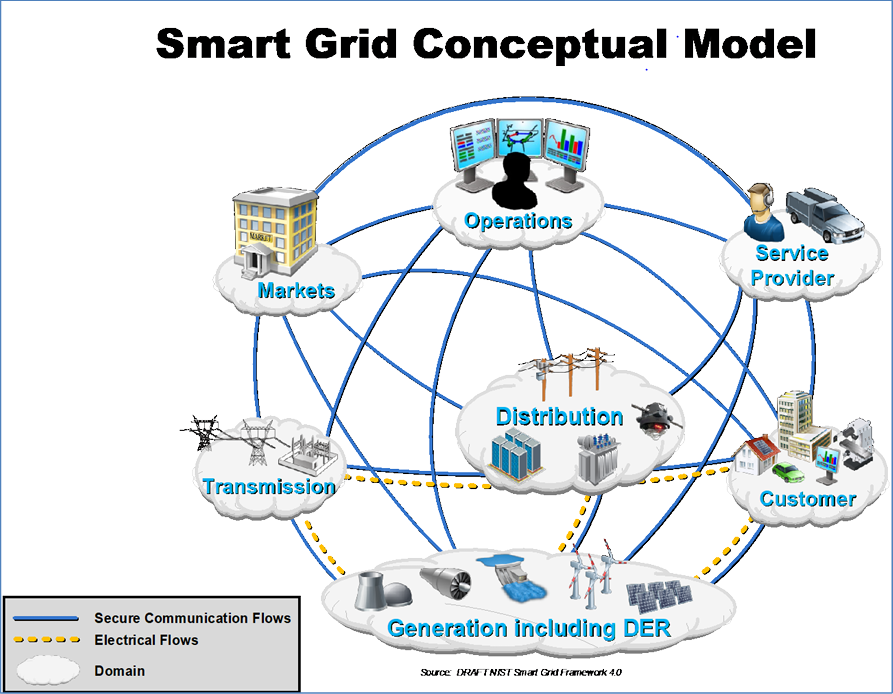
\includegraphics[width=\textwidth]{figures/nist.PNG}
	\caption{The NIST Conceptual Model for SG \cite{gopstein2021nist}}
	\label{fig:example}
\end{figure}
\begin{table}[h]
    \centering
 %%ffffff
    
% \begin{tabularx}{\textwidth}{|X|X|}
% \hline
% \textbf{Domain} & \textbf{Roles/Services in the Domain} \\
% \hline
% 1 Customer & The end users of electricity. May also generate, store, and manage the use of energy. Traditionally, three customer types are discussed, each with its own sub-domain: residential, commercial, and industrial. \\
% \hline
% 2 Markets & The facilitators and participants in electricity markets and other economic mechanisms used to drive action and optimize system outcomes. \\
% \hline
% 3 Service Provider & The organizations providing services to electrical customers and to utilities. \\
% \hline
% 4 Operations & The managers of the movement of electricity. \\
% \hline
% 5 Generation Including DER & The producers of electricity. May also store energy for later distribution. This domain includes traditional generation sources and distributed energy resources (DER). \\
% \hline
% 6 Transmission & The carriers of high voltage electricity over long distances. May also store and generate electricity. \\
% \hline
% 7 Distribution & The distributors of electricity to and from customers. May also store and generate electricity. \\
% \hline
% \end{tabularx}
\begin{tabular}{|p{0.15\textwidth}|p{0.8\textwidth}|}
    \hline
    \textbf{Domain} & \textbf{Roles/Services in the Domain} \\
    \hline
    1 Customer & The end users of electricity. May also generate, store, and manage the use of energy. Traditionally, three customer types are discussed, each with its own sub-domain: residential, commercial, and industrial. \\
    \hline
    2 Markets & The facilitators and participants in electricity markets and other economic mechanisms used to drive action and optimize system outcomes. \\
    \hline
    3 Service Provider & The organizations providing services to electrical customers and to utilities. \\
    \hline
    4 Operations & The managers of the movement of electricity. \\
    \hline
    5 Generation Including DER & The producers of electricity. May also store energy for later distribution. This domain includes traditional generation sources and distributed energy resources (DER). \\
    \hline
    6 Transmission & The carriers of high voltage electricity over long distances. May also store and generate electricity. \\
    \hline
    7 Distribution & The distributors of electricity to and from customers. May also store and generate electricity. \\
    \hline
    \end{tabular}
    \caption{Domains and their associated roles/services \cite{gopstein2021nist}}
    \label{table:domains}
\end{table}
\section{Benefits of Smart Grid}  
\section{Motivations and Challenges towards Smart Grid }  
\section{risk Smart Grid }  

\section{Related Works}
\section{Synthesis and Discussion}
\section*{Conclusion}
